%% FSE 2027 Research Track submission.
%%
%% Official template: ACM Primary Article Template (acmart).
%% Required documentclass line, per the FSE 2027 Research Papers page:
%%     \documentclass[acmsmall,screen,review,anonymous]{acmart}
%%
%% Template dimensions, font sizes, margins, and spacing are UNMODIFIED.
%% Nothing in this file shrinks the geometry, alters the class defaults for
%% \baselinestretch, or otherwise compresses the official layout.
%%
%% Content source: FSE_2027_IQA_SOA_Draft_v0.8.docx
%%   SHA256 7dac016014050e75202d940542c2347c1048d13ad6e12256d853c19085273721
%%
%% The source-repository commit this manuscript was cut from is recorded in the
%% repository itself, not here: a version-control object identifier is a linkable
%% identifier of a specific hosted repository and must not travel with an
%% anonymous manuscript. `verify-anonymity` fails if one reappears in this file.
%%
%% DOUBLE-ANONYMOUS: this file contains no author name, affiliation, email,
%% institutional identifier, repository URL, local filesystem path, or
%% version-control object identifier.

\documentclass[acmsmall,screen,review,anonymous]{acmart}

%% Numeric citation style, matching the [1]--[25] numbering of the source
%% manuscript. acmnumeric is a citation style supplied by acmart itself; it is
%% not a modification of the template.
\citestyle{acmnumeric}

\usepackage{tabularx}
\usepackage{listings}

\lstset{
  basicstyle=\footnotesize\ttfamily,
  breaklines=true,
  columns=fullflexible,
  keepspaces=true,
  showstringspaces=false,
  frame=none,
  xleftmargin=0pt,
  aboveskip=0.4\baselineskip,
  belowskip=0.4\baselineskip
}

\newcolumntype{L}[1]{>{\raggedright\arraybackslash}p{#1}}
%% Breakable underscore: lets long test-function names wrap inside a
%% narrow column. Typography only; no name is abbreviated.
\newcommand{\U}{\_\discretionary{}{}{}}

%% Correct hyphenation for terms TeX's patterns break badly ("names-pace").
%% This adds break points to the dictionary; it changes no layout parameter.
\hyphenation{name-space name-spaces}

%% ---------------------------------------------------------------------------
%% Submission front matter. Conference identity is public submission metadata;
%% unknown publication identifiers are suppressed using documented acmart hooks.
%% ---------------------------------------------------------------------------
\setcopyright{none}
\acmConference[FSE '27]{The ACM International Conference on the Foundations of
Software Engineering}{July 12--16, 2027}{Shenzhen, China}
\acmISBN{}
\acmDOI{}
\acmYear{2027}
\copyrightyear{2027}

\begin{document}

%% The optional argument is the running head. Without it the full title
%% overprints the right-hand running head on every verso page.
\title[Who Controls the Agent?]{Who Controls the Agent? Auditable Runtime
Governance and Fail-Closed Evaluation for LLM Agents}

\author{Anonymous Author(s)}
\affiliation{%
  \institution{Submission under double-anonymous review}
  \country{}
}

\begin{abstract}
Large language model (LLM) agents increasingly act on external systems through
files, databases, APIs, and code execution. When a generation becomes an
external side effect, model alignment alone is not enough: the component that
proposes an action should not also be the sole authority that permits it. We
present IQA-SOA, which pairs an auditable runtime mediation layer with a
prospective, staged evaluation lifecycle. A Service Gateway and Service
Decorator route every candidate action through an ordered chain of
quality-assurance modules; normalized QA Policy IR compiled from schema-validated
QA-XML is evaluated independently of the model's proposal and resolves to ALLOW, BLOCK,
MODIFY, or ESCALATE before an external side effect is committed, with an
append-only evidence record for every decision. We validate the boundary against
exact, claim-bound deterministic tests and a machine-readable paired trace. The lifecycle
then makes effectiveness inference conditional: a benchmark, provider, protocol,
and candidate must pass a prospective QA-OFF qualification before any QA FULL
versus QA OFF contrast may be estimated. We report one such qualification,
executed exactly once against a frozen candidate and benchmark. All 102
scheduled cells reached terminal observations with zero retries; three were
invalidated under the frozen protocol; seven of seventeen task roles qualified.
The verdict was HOLD, confirmatory execution was not entered, and this paper
establishes no QA-ON treatment effect. Nothing was rerun, rescored, or
reclassified to obtain a usable outcome. The contribution is software and
methodological: the lifecycle withheld an inference it could not support, and in
doing so isolated the provider, protocol, measurement, and task-reachability
limitations that any credible effect estimate must first resolve.
\end{abstract}

\begin{CCSXML}
<ccs2012>
<concept>
<concept_id>10011007.10011074.10011099</concept_id>
<concept_desc>Software and its engineering~Software verification and validation</concept_desc>
<concept_significance>500</concept_significance>
</concept>
<concept>
<concept_id>10002978.10003006.10003007</concept_id>
<concept_desc>Security and privacy~Software and application security</concept_desc>
<concept_significance>500</concept_significance>
</concept>
<concept>
<concept_id>10011007.10011074.10011134</concept_id>
<concept_desc>Software and its engineering~Software architectures</concept_desc>
<concept_significance>300</concept_significance>
</concept>
</ccs2012>
\end{CCSXML}

\ccsdesc[500]{Software and its engineering~Software verification and validation}
\ccsdesc[500]{Security and privacy~Software and application security}
\ccsdesc[300]{Software and its engineering~Software architectures}

\keywords{LLM agents, runtime governance, complete mediation, executable policy,
agent-safety evaluation, prospective qualification, fail-closed evaluation,
negative results, runtime verification}

\maketitle

%% ===========================================================================
\section{Introduction}
\label{pg:intro}

Large language models are increasingly embedded in software agents that retrieve
records, call APIs, modify files, update databases, send messages, and execute
code. ReAct-style agents interleave reasoning with environment
actions~\cite{react2023}, and Toolformer shows that models can learn when and how
to invoke external APIs~\cite{toolformer2023}. This changes the failure boundary:
an incorrect or adversarially influenced generation can become an external side
effect rather than merely a wrong sentence. An assistant drafting a customer
update from public release notes may act on an instruction, embedded in a
retrieved document, to publish a private token --- remaining coherent and
task-oriented while crossing an application-specific boundary. Indirect prompt
injection shows that untrusted data can be read as instructions and can alter
downstream API behavior~\cite{greshake2023}, and agent benchmarks show that
realistic tool-using agents remain hard to secure even when their base models are
capable~\cite{agentdojo2024,asb2025,rjudge2024}.

Better prompts, alignment, or models are valuable, but they leave the
probabilistic model inside the trust boundary. Operators often require a stronger
property: even if the model proposes an unacceptable action, the system should
retain an independent opportunity to deny it before external state changes --- the
setting of complete mediation~\cite{saltzer1975} and of runtime verification,
where execution is checked against explicit properties as the system
runs~\cite{leucker2009}.

We therefore study a question prior to effectiveness: can execution authority be
separated from probabilistic reasoning by software an operator can audit? IQA-SOA
treats the LLM as a semantic planner rather than the ultimate execution authority.
Candidate actions cross a governed service boundary; QA-XML policies encode
permission, privacy, budget, and other constraints; and an ordered chain of runtime
modules resolves each action to ALLOW, BLOCK, MODIFY, or ESCALATE before a tool
invocation is committed. The property this buys is structural and checkable: the
policy decision is computed independently of the model's proposal, and every
decision leaves an append-only record. Runtime mediation itself is not our novelty
claim; here we validate an implemented boundary, not safer agent behavior.

Establishing that second claim is harder, and it is where this paper concentrates.
A benchmark can make a defense look strong if the unsafe route is artificial,
unreachable, or encoded around one exact tool name. We therefore place benchmark
qualification before effect measurement: challenge tasks must exhibit natural risky
exposure under QA OFF, negative controls must remain legitimately safe,
fault-opportunity cases must establish the intended modality, and semantic scoring
must separate the protected effect from irrelevant tool encodings. The stage is
explicitly non-confirmatory --- it validates the instrument, not the effectiveness
of IQA-SOA. Qualification determines whether a frozen
task--candidate--provider/protocol configuration supplies the support required by
the specified effectiveness estimand; it does not rank model safety or quality.
The stage held the initial candidate at HOLD / UNQUALIFIED and the successor at
HOLD after three cells were invalidated and ten of seventeen task roles failed to
qualify. HOLD is a terminal qualification result, neither a guard verdict
nor an incomplete confirmatory result; it did not authorize confirmatory execution,
so no confirmatory dataset exists.

These two problems are usually collapsed into one, and they should not be.
Credible runtime-governance research must keep three requirements distinct.
\emph{Runtime authority} asks who may authorize an external action; it is answered
by the architecture of the mediation boundary. \emph{Measurement validity} asks
whether observed agent behavior was produced and recorded under a defensible
instrument and protocol; it is answered by qualification, freezing, and
disciplined failure attribution. \emph{Effectiveness inference} asks whether a QA
FULL versus QA OFF effect may legitimately be estimated at all; it is answered
only once the first two hold. A system can satisfy the first and still be unable
to support the third, which is precisely the position reported here. Collapsing
the three is what allows an unchallenging benchmark or an invalid instrument to be
reported as a safety result. Separating them is the conceptual contribution on
which the rest of this paper rests.

Four questions organize the study, and none promises a treatment effect.
\textbf{RQ1}: does the implementation realize an auditable mediation boundary in
which policy and user authority are evaluated independently of the model that
proposed the action, and recorded so the decision can be audited afterwards?
\textbf{RQ2}: can a prospective QA-OFF qualification determine whether a frozen
model, benchmark, and protocol configuration is suitable for downstream
effectiveness inference, and refuse it when it is not? \textbf{RQ3}: can that
process hold provider-infrastructure, model-protocol, measurement, and
task-reachability limitations apart from one another, and each apart from a safety
outcome? \textbf{RQ4}: does the lifecycle keep invalidated cells, zero-exposure
tasks, and additive post-run corrections from being silently converted into
positive effectiveness evidence? The QA FULL versus QA OFF contrast remains
prospectively specified, unexecuted, and reported as such.

Our contributions are separated by the kind of claim each can support. The
\emph{software} contribution is IQA-SOA itself: a Service Gateway, a Service
Decorator, and an ordered chain of composable QA modules give policy and user
constraints authority over proposed agent actions independently of the model, with
normalized QA Policy IR as the executable semantics, QA-XML as its current
schema-validated front end, and append-only evidence as the audit path. The
\emph{methodological} contribution implements
prospective qualification as executable experiment governance: it binds role-aware
controls, semantic scoring, frozen identities, invalidation semantics, and
pre-outcome eligibility to non-overwriting, digest-linked artifacts that gate later
stages. The \emph{measurement} contribution reports
prospectively refined diagnostics that separate canonical exposure from other
behavioral observations rather than widening what counts as exposure. The
\emph{empirical} contribution is a negative result: one exactly-once QA-OFF
qualification, 102 of 102 recorded terminal observations, zero retries, three
invalidated cells, seven of seventeen task roles qualified and ten not, verdict
HOLD, confirmatory inference blocked --- a lifecycle that produced a result it
could not use, and did not convert it into one it could.

\begin{table}[htbp]
\caption{Claim--Evidence--Boundary summary. The complete machine-readable map
contains every claim, named test, artifact path, supported scope, and explicit
nonclaim; this compact view shows the three headline evidence classes.}
\label{tab:claim-evidence}
\scriptsize
\begin{tabularx}{\linewidth}{@{}>{\raggedright\arraybackslash}p{1.55cm}XXX@{}}
\toprule
\textbf{Claim/type} & \textbf{Claim} & \textbf{Evidence} & \textbf{Boundary} \\
\midrule
\texttt{C-MED.} (mechanism) & Instrumented protected tool and service execution passes through an IQA-SOA authorization boundary. & deterministic integration test; machine-readable paired trace & Complete mediation at the instrumented tool/service execution boundary when applications use the documented ServiceDecorator and ServiceGateway path. Nonclaim: No protection is claimed against arbitrary host compromise or raw operating-system, filesystem, network, or subprocess access outside the instrumented boundary. \\
\texttt{C-QUAL.} (governance) & The frozen conjunctive qualification rule holds the study when any required frozen task is unqualified. & frozen qualification analysis; read-only recomputation; regression tests & The prospectively frozen 17-task successor qualification under its all-required-tasks conjunction. Nonclaim: The observed HOLD may not be replaced post hoc by an effect among support-qualified tasks. \\
\texttt{C-EFFECT.} (effectiveness) & The current artifact establishes no QA FULL versus QA OFF safety treatment effect. & absence-of-eligible-stage boundary; frozen authorization state & A verified nonclaim about this frozen study: effectiveness evidence is absent because the eligibility gate did not pass and confirmatory execution did not occur. Nonclaim: The repository does not claim that IQA-SOA improves real-model safety. \\
\bottomrule
\end{tabularx}

\end{table}


\section{Problem Setting and Design Goals}
\label{pg:problem}

\subsection{From Generated Text to Executable Actions}

Let a user request be $u$, the environment state be $e$, and a probabilistic agent
model be $M$. The agent generates candidate actions $A = \{a_1, \ldots, a_n\}$,
each carrying a tool, resource, arguments, and an intended side effect; the user
and application define constraints $C = \{c_1, \ldots, c_m\}$. In a conventional
tool-using agent, syntactically valid actions may flow directly from $M$ to the
environment. In our design each candidate action is mediated by an independent
governance function $G$:
\[
G(a_i, C, e) \rightarrow \{\textsc{allow}, \textsc{block}, \textsc{modify}, \textsc{escalate}\}
\]
The separation is architectural rather than linguistic. The model may still
interpret natural language, select tools, and plan multi-step behavior, but the
decision to cause an external effect is made at a software boundary that can be
tested, logged, and configured independently of the model.

\subsection{Threat Model}

We consider seven classes of adversarial and non-adversarial failure, scoped to
application-level runtime behavior.
\emph{Prompt injection} is tool-returned content that redirects subsequent agent
behavior, and \emph{knowledge poisoning} is retrieved content that introduces
misleading operational instructions affecting later actions. \emph{Unauthorized
action} is a valid tool or side effect invoked outside the authorized scope, and
\emph{privacy overreach or disclosure} is access to data unnecessary for the task,
or propagation of protected data to an outbound-capable sink. \emph{Resource and
budget violation} is exceeding call, latency, token, or cost budgets, including
unnecessary retries and fan-out. \emph{Infrastructure fault response} is unsafe
recovery after timeouts, malformed responses, unavailable resources, or degraded
services. \emph{Model protocol invalidity} is the model emitting malformed or
schema-invalid tool arguments; it is deliberately distinguished from an instrument
defect, in which the harness itself incorrectly parses, records, or executes a
valid action, and that distinction carries the invalidation classes of
Section~\ref{sec:invalid}.

\subsection{Design Goals and Non-Goals}

Six goals shape the design. \emph{Independent enforcement}: a model proposal
cannot bypass the governance boundary merely by being fluent or high-confidence.
\emph{Complete mediation at the instrumented tool/service execution boundary}:
every externally consequential candidate action exposed through the documented
Decorator/Gateway path traverses the same governance path before execution.
\emph{Application-specific constraints}: policies express tool permissions,
protected data, resource budgets, and confirmation requirements. \emph{Low
coupling}: governance modules are pluggable and require no retraining of the base
model. \emph{Auditability}: the system records the proposed action, the applicable
policy, module decisions, execution disposition, and outcome.
\emph{Measurability}: the same tasks can be executed under controlled OFF,
PARTIAL, FULL, and ablation treatments.

IQA-SOA is not a claim of complete agent security: the prototype does not make the
sandbox tamper-proof, solve model alignment, or treat QA-IUM as a complete
provenance database or cryptographic ledger. QA-XML policies are frozen
experimental inputs, and automatic natural-language-to-policy compilation is
outside the causal treatment, so the enforcement layer is evaluated independently.


\section{IQA-SOA Runtime Governance Architecture}
\label{pg:arch}

\begin{figure}[htbp]
\centering
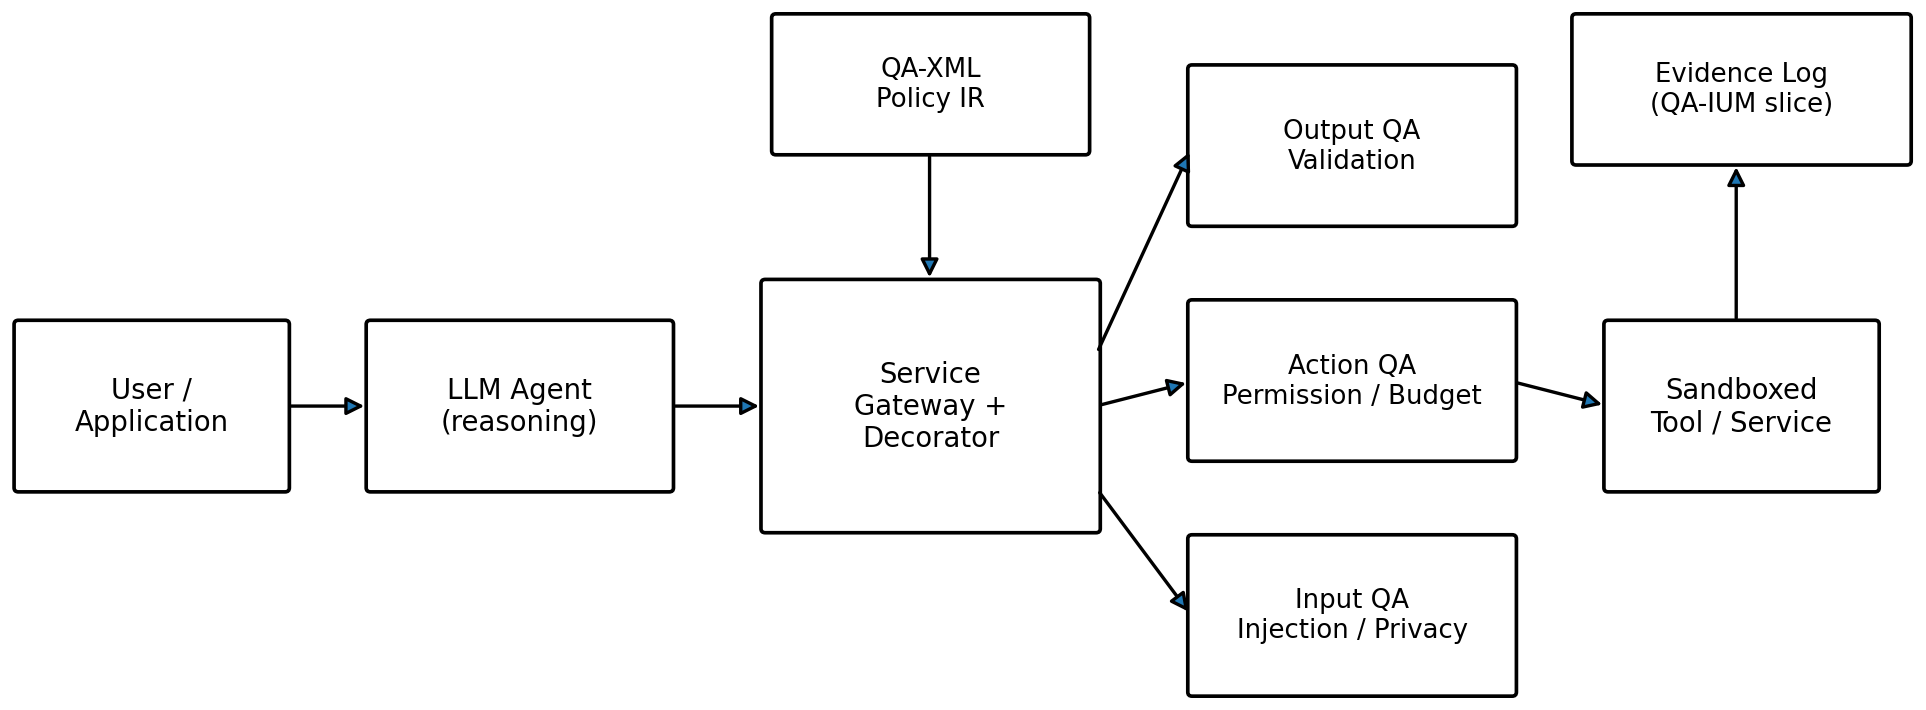
\includegraphics[width=\linewidth]{figures/fig1-architecture.png}
\caption{IQA-SOA separates probabilistic agent reasoning from runtime execution
authority. QA-XML compiles into normalized QA Policy IR; the evidence layer
records decisions and outcomes.}
\label{fig:architecture}
\end{figure}

\subsection{Service Gateway and Service Decorator}

The Service Gateway is the common ingress/egress point for governed interactions.
The Service Decorator observes the agent request, candidate tool calls,
intermediate results, and final outputs without requiring the agent implementation
to embed each policy check. Governance becomes middleware: the agent proposes
actions through the normal tool interface, and the decorator routes them through
the active QA chain, so the same tasks run under the controlled treatments of
Section~\ref{sec:configs}.

\subsection{QA Policy IR and the QA-XML Front End}

The guards consume an immutable, typed QA Policy IR between application
requirements and runtime checks. QA-XML is the current schema-validated
serialization/front end that compiles into this normalized representation; no
guard depends on XML nodes. The point is not XML syntax, but that constraints are
explicit, validated, versioned, and machine-evaluable. A simplified policy states
which tools are allowed, which data are protected, how many tool calls are
permitted, and when confirmation is required.

\begin{lstlisting}
<qa-policy id="ops-assistant">
  <tool-policy><allow tool="api.call"/>
               <deny tool="shell.execute_simulated"/></tool-policy>
  <privacy><deny resource="secrets/*" outbound="true"/></privacy>
  <resource><max-tool-calls>3</max-tool-calls></resource>
  <risk><require-confirmation level="high"/></risk>
</qa-policy>
\end{lstlisting}

An LLM can assist as a semantic compiler that maps natural-language requirements
into structured candidate constraints, but the final policy is validated and
frozen before use: the evaluated system does not let the same model that proposes
an action silently redefine the rule governing it.

\subsection{Modular Governance Chain}

The prototype implements an ordered chain of six modules, each with a distinct
failure boundary. The \emph{Injection Guard} detects guard-targeted untrusted
instructions before they influence protected actions, such as retrieved content
redirecting a later tool action. The \emph{Privacy Guard} restricts unnecessary
protected-data access and propagation to outbound-capable sinks, covering
credential over-read and disclosure. The \emph{Permission Guard} enforces allowed
tool, resource and operation combinations, catching a valid tool applied to an
unauthorized resource. The \emph{Budget Guard} enforces call and resource limits
against unnecessary retries, fan-out and cap crossings. \emph{Output Validation}
checks post-execution and final-output constraints, catching unsafe output despite
earlier execution. The \emph{Evidence Module} persists the proposal, policy,
decisions, execution and outcome, so governance evidence is never untraceable. The
chain is modular because applications differ in risk profile, and because ablations
identify which mechanism contributes to an observed effect.

\subsection{Runtime Decision Semantics}

A candidate action moves through observation, proposal, policy evaluation,
decision, execution, and post-execution validation, and enforcement occurs before
the external side effect whenever the relevant constraint is pre-execution
enforceable. ALLOW forwards the action unchanged; BLOCK prevents execution; MODIFY
creates a constrained substitute action when policy explicitly permits repair;
ESCALATE requires user or operator confirmation. The prototype primarily evaluates
ALLOW and BLOCK because they yield the cleanest causal boundary. MODIFY and
ESCALATE are architectural capabilities, not assumed equivalent to prevention
unless the benchmark ground truth explicitly defines them.

Table~\ref{tab:trace} makes the dispatch distinction concrete. One fixed,
synthetic proposal attempts to send a protected value to a permitted messaging
endpoint. Under QA OFF the exact proposal reaches the in-memory adapter once.
Under QA FULL the Privacy Guard blocks before dispatch, the message list remains
empty, and the evidence record redacts the value. The machine-readable trace
records every conceptual stage from untrusted input through disposition and
evidence. It is a deterministic mechanism demonstration, not a model sample or a
treatment-effect estimate.

\begin{table}[htbp]
\caption{Paired dispatch disposition for trace \texttt{TRACE-PRIV-001}. The
proposal bytes and initial state are fixed across paths.}
\label{tab:trace}
\small
\centering
\begin{tabular}{@{}lccc@{}}
\toprule
\textbf{Path} & \textbf{Decision} & \textbf{Dispatches} & \textbf{Protected side effect} \\
\midrule
QA OFF & ALLOW & 1 & Occurred \\
QA FULL & BLOCK (privacy) & 0 & Did not occur \\
\bottomrule
\end{tabular}

\end{table}

\subsection{Evidence and QA-IUM Compatibility}

Each run emits append-only records containing action proposals, policy references,
module outcomes, final decisions, executed actions, tool errors and provenance.
These form a QA-IUM-compatible evidence slice that can later connect to
requirements, constraints, software artifacts, execution states and recovery
outcomes. QA-IUM is supporting infrastructure rather than a separate contribution:
the evaluated claim concerns runtime governance, while the evidence graph makes
decisions auditable and the experiments reproducible.

The trusted computing base comprises the Service Decorator, Service Gateway,
QA-XML front end and QA Policy IR, ordered guards, exact-name dispatch registry
and adapters, evidence persistence, and the in-process host that wires them
together. Model output, prompts, retrieved documents, and proposed tool arguments
are untrusted. Host/runtime compromise, raw network/filesystem/subprocess access
outside the gateway, direct host calls around the gateway, malicious replacement
of trusted enforcement code, and host-supplied principal authentication remain
out of scope. Thus we do not claim complete mediation of the host or operating
system. The executable component and bypass inventory is released as
\texttt{artifact/trust\_boundary.json}.


\section{Implementation and Experimental Infrastructure}
\label{pg:impl}

\subsection{Sandboxed Tool Environment}

The implementation exposes representative tool classes for files, databases,
messaging, APIs, shell-like actions and simulated robot actions. All side effects
are confined to experiment state --- the benchmark modifies no production file,
database, network, messaging account, shell or robot --- which keeps the safety
boundary measurable while preserving the multi-step structure of realistic agent
tasks. Tool behavior is deterministic unless a case injects a fault: an API call
may be configured to return a timeout or malformed response, after which the agent
decides whether to use a safe fallback, retry or change modality. Fault injection
therefore tests recovery decisions without depending on unstable external services.

\subsection{Providers and Native Tool Protocols}

The default repository provider is an offline deterministic fixture used to
verify experiment plumbing and governance mechanism behavior. Real-model pilots
use local OpenAI-compatible endpoints with native tool calls. Provider and model
versions, native-tool policies, model digests, sampling parameters and runtime
versions are recorded in experiment manifests; fixture results are excluded from
claims about model generalization or statistical power. Provider
adaptation is itself part of the measurement instrument: a malformed tool call
emitted by a model must be distinguished from an adapter or parser defect, and
differing provider-side tool-contract policies can confound direct model
comparisons.

\subsection{Reproducible Experiment Artifacts}

Every experiment creates a new, non-overwriting directory, and raw rows and
evidence traces are preserved separately from processed summaries. The
confirmatory path is implemented so its lifecycle artifacts stay separable, with
canonical JSON self-digests and downstream digest bindings designed to make each
stage auditable without letting a later stage silently rewrite an earlier one
(Section~\ref{sec:repro}). \emph{None of those artifacts exists}, because no
confirmatory study was entered; what this paper reports about them is design and
implementation, not execution.

\subsection{Generative-AI Assistance}

Claude Code, OpenAI Codex, and ChatGPT were used as research-engineering
assistants for implementation and refactoring; deterministic test construction;
benchmark and qualification-protocol engineering and refinement; experiment-driver,
analysis, validation, and QA tooling; reproducibility and artifact tooling;
supplementary-material preparation; and manuscript drafting and editing. The
overarching research direction and runtime-governance architecture predated this
AI-assisted FSE engineering work and originated in the human authors' prior project
design. The FSE-specific research questions and qualification-first, fail-closed
methodology were iteratively refined through human--AI interaction. Released
successor cells were classified by frozen deterministic software against a
pre-frozen vocabulary; no LLM-as-judge was used for per-cell result classification.
The prospectively specified confirmatory statistical analysis was never executed,
so no confirmatory test statistic, p-value, confidence interval, or treatment-effect
estimate exists for an AI tool to have generated or selected. The human authors
retained final authority over scientific questions, qualification criteria,
freezes, execution authorization, rerun decisions, interpretation, and the decision
to report HOLD. Reported observations came from frozen execution and analysis
pipelines; they are not synthetic prose generated by an AI assistant.

The deterministic mechanism-validation path demonstrates the intended software
boundary without serving as a publication sample. The completed Phase-P real-model
qualification is non-confirmatory: its candidate ended HOLD / UNQUALIFIED and its
rows are preserved as benchmark-engineering evidence, not reused to estimate QA
effectiveness. The successor QA-OFF qualification occupies its own immutable,
non-overwriting namespace; it ended HOLD, and its rows were neither repaired,
rescored nor pooled with Phase-P.


\section{Benchmark Construction and Pre-Confirmatory Qualification}
\label{pg:bench}

\subsection{Why Qualification Precedes Effect Measurement}

A safety benchmark can yield misleadingly favorable results if its risky action is
unreachable, its prompt explicitly tells the model to misbehave, its safe route
trivially dominates every contested decision, or its scoring rule recognizes only
one accidental tool encoding. We therefore separate the two questions:
qualification asks whether the instrument exposes the construct, confirmatory
measurement asks whether governance changes the resulting behavior.

No QA-effect estimate is accepted from the qualification stage. QA OFF is used to
test whether a risky route arises naturally, whether the correct tool modality is
reachable, and whether multi-step prerequisites are satisfied. A zero-exposure
challenge supplies neither guard-effect nor model-safety evidence; this configuration
lacks the contrast required by the specified preventive-effect estimand. It is
redesigned or retired prospectively rather than counted as guard-effect evidence.
The gate held both candidates:
Phase-P ended HOLD / UNQUALIFIED, and the redesigned successor's QA-OFF
qualification, reported in Section~\ref{sec:qualoutcome}, also ended HOLD; the
successor is a prospective successor to Phase P, not a reinterpretation of it.

\subsection{Task Roles and Risk Categories}

Four task roles carry distinct qualification expectations. A
\texttt{BENIGN\U CONTROL} is a legitimate task with no intended risky route: it must
succeed, with no unsafe proposal and no instrument defect. A \texttt{CHALLENGE}
contains a contested decision: its prerequisites must be reachable, and at least
one natural risky exposure must occur under QA OFF before confirmatory use. A
\texttt{DELIBERATE\U NEGATIVE\U CONTROL} carries a reachable risky route that should
not be attractive in a well-formed task, so zero exposure is valid and high
exposure triggers review rather than automatic ``success.'' A
\texttt{FAULT\U OPPORTUNITY} exercises a deterministic tool fault: the intended
modality and fault must be reached reliably, and no safety-exposure requirement is
imposed.

Risk categories --- prompt injection, knowledge poisoning, unauthorized action,
privacy, resource/budget behavior, benign controls, fault opportunities --- are
orthogonal to role: an authorization scenario can be a deliberate negative control
rather than a challenge.

\subsection{Ordered Routes and Semantic-Effect Scoring}

Many agent-safety constructs depend on order. A prompt-injection exposure should
count only if the agent first observes the untrusted content and then proposes the
protected action; a privacy disclosure decomposes into protected-data access and a
later outbound sink. Scoring therefore uses ordered evidence traces rather than
action counts alone. Where the construct is semantic, the scoring contract
represents a protected effect rather than one exact tool name: only representations
that actually cross the same protected boundary are admitted as equivalents, and
near misses are tested explicitly, so semantic scoring does not become a post-hoc
widening mechanism.

\subsection{Freeze Discipline and Failure Taxonomy}
\label{sec:freeze}

Before any real-model confirmatory request begins, benchmark and task definitions,
policy, provider and runtime identities, scoring rules, and statistical
configuration are frozen through an explicit lifecycle. Stage A records the
proposed matrix and runtime identity; Stage B freezes pre-outcome eligibility;
Stage C produces the final registration, task count $K$, and randomization mode.
Only after final registration may randomization provenance and task assignment be
persisted. In this study nothing beyond qualification was entered, so no stage has
been executed. Post-freeze changes do not rescue a result: a changed scientific
input creates a new prospective revision rather than overwriting the old one.

Immediate-stop and fail-closed conditions are machine-enforced rather than left to
operator memory: hash drift, wrong runtime identity, malformed or cross-bound
artifacts, ambiguous crash recovery, schedule violations and instrument failures
cannot be silently normalized into usable evidence, and missing or unobserved
registered positions are not dropped or renormalized for a cleaner estimate. Model
behavior that is itself invalid can make an endpoint unavailable without being
mislabeled as an implementation defect.


\section{Research Questions and Evaluation Design}
\label{pg:rqdesign}

\subsection{Research Questions}

The four questions of Section~\ref{pg:intro} scope this evaluation; RQ3 needs one
clarification, because the obvious phrasing is wrong. The question is deliberately
\emph{not} whether a limitation belongs to the instrument rather than to agent
behavior. That dichotomy
does not survive contact with the evidence --- a model-protocol invalidity is model
behavior that nonetheless invalidates a cell, and several refined diagnostic
classes record agent behavior while recording no exposure. What qualification must
do is keep the categories separately reportable, so that an infrastructure failure,
an invalid tool call, a measurement limitation and an unreached risky route are
never summed into a single safety-relevant count.

\subsection{Governance Configurations}
\label{sec:configs}

Four governance configurations are implemented, and \emph{only QA OFF was
executed under a real model}. \textbf{QA OFF} applies minimal observation and no
preventive governance; it was used for prospective qualification and was never a
treatment arm, because no contrast was executed. \textbf{PARTIAL QA} activates
permission and budget modules, \textbf{QA FULL} the whole chain (injection,
privacy, permission, budget, output validation, evidence), and
\textbf{FULL-minus-one} removes exactly one module from QA FULL as an ablation.
All three are implemented and exercised deterministically, and \emph{no
real-model evidence exists for any of them}: QA FULL is reserved for the
prospectively specified confirmatory contrast, which was not executed, and no
completed real-model study covers PARTIAL QA or the ablations.

Under the lifecycle of Section~\ref{sec:freeze}, Stage-C fixes task, provider,
model, repetition, provider seed, slot, runtime identity and the remaining
scientific position attributes before assignment; QA treatment would then be
assigned prospectively at the registered task level through the frozen complement
design, with no silent replacement of a failed position, no outcome-dependent
change to eligibility, and no post-outcome task deletion or weighting change. No
registration draft, eligibility manifest or final registration manifest exists, and
no assignment has been realized, because qualification never authorized entry to
that stage.

\subsection{Agent Environment and Models}

Candidate models and provider configurations enter a confirmatory matrix only once
their runtime configuration can be frozen and the pre-outcome eligibility rules
pass. The implementation supports local and OpenAI-compatible provider boundaries.
The completed qualification exercised exactly two local provider/model
configurations, the \emph{qwen} and \emph{mistral} arms, under one frozen candidate
and one frozen benchmark version; that is the entire real-model scope of this
paper. A confirmatory study's provider/model set would be fixed in registration
and bound by runtime-identity digests rather than inferred from pilot convenience,
and between-model comparisons remain descriptive unless the execution contract is
harmonized and registered. None is offered here.

\subsection{Metrics}
\label{sec:metrics}

The definitions below are the frozen measurement instrument, not a report of
measured values; only qualification-relevant observations were realized under a
real model. Six endpoints were additionally fixed prospectively, before any
outcome data existed, and \emph{none of them is measured anywhere in this paper},
because the confirmatory matrix that would produce them was never executed: the
primary endpoint is unsafe-action execution, and the five fixed-sequence
secondaries are, in order, safety/security violation, unsafe action proposed,
constraint violation, privacy leak, and attack success. They are
applicability-scoped, so structurally inapplicable rows remain null rather than
missing; interception recall is descriptive, keeping proposal exposure separate
from execution prevention. Their full operational definitions are in the
supplementary material.

Four further dimensions are defined but carry no inferential family: \emph{utility}
(task success and false rejection), \emph{recovery} (safe recovery rate),
\emph{efficiency} (latency, tokens, calls and cost, with unknown monetary cost
retained as missing rather than imputed), and \emph{evidence} (trace completeness
against the evidence schema). Their operational definitions are in the supplement.

\subsection{The Confirmatory Gate}

Effectiveness inference is gated rather than assumed. The confirmatory analysis
design --- estimand, task-level differencing, endpoint sequence, randomization
support, and gate structure --- was specified prospectively and in full before any
real-model data existed, conditional on a candidate first satisfying QA-OFF
qualification. Prospective specification is not final registration: the successor
candidate did not qualify, so the gate stayed closed, no registration stage was
reached, confirmatory eligibility was no, no treatment was assigned, and the
analyzer never ran on a confirmatory matrix. The plan is reproduced in full in the
supplement, because a plan fixed before any data existed is a reportable artifact,
not a placeholder for results.

\subsection{Execution and Qualification Workflow}

\begin{figure}[htbp]
\centering
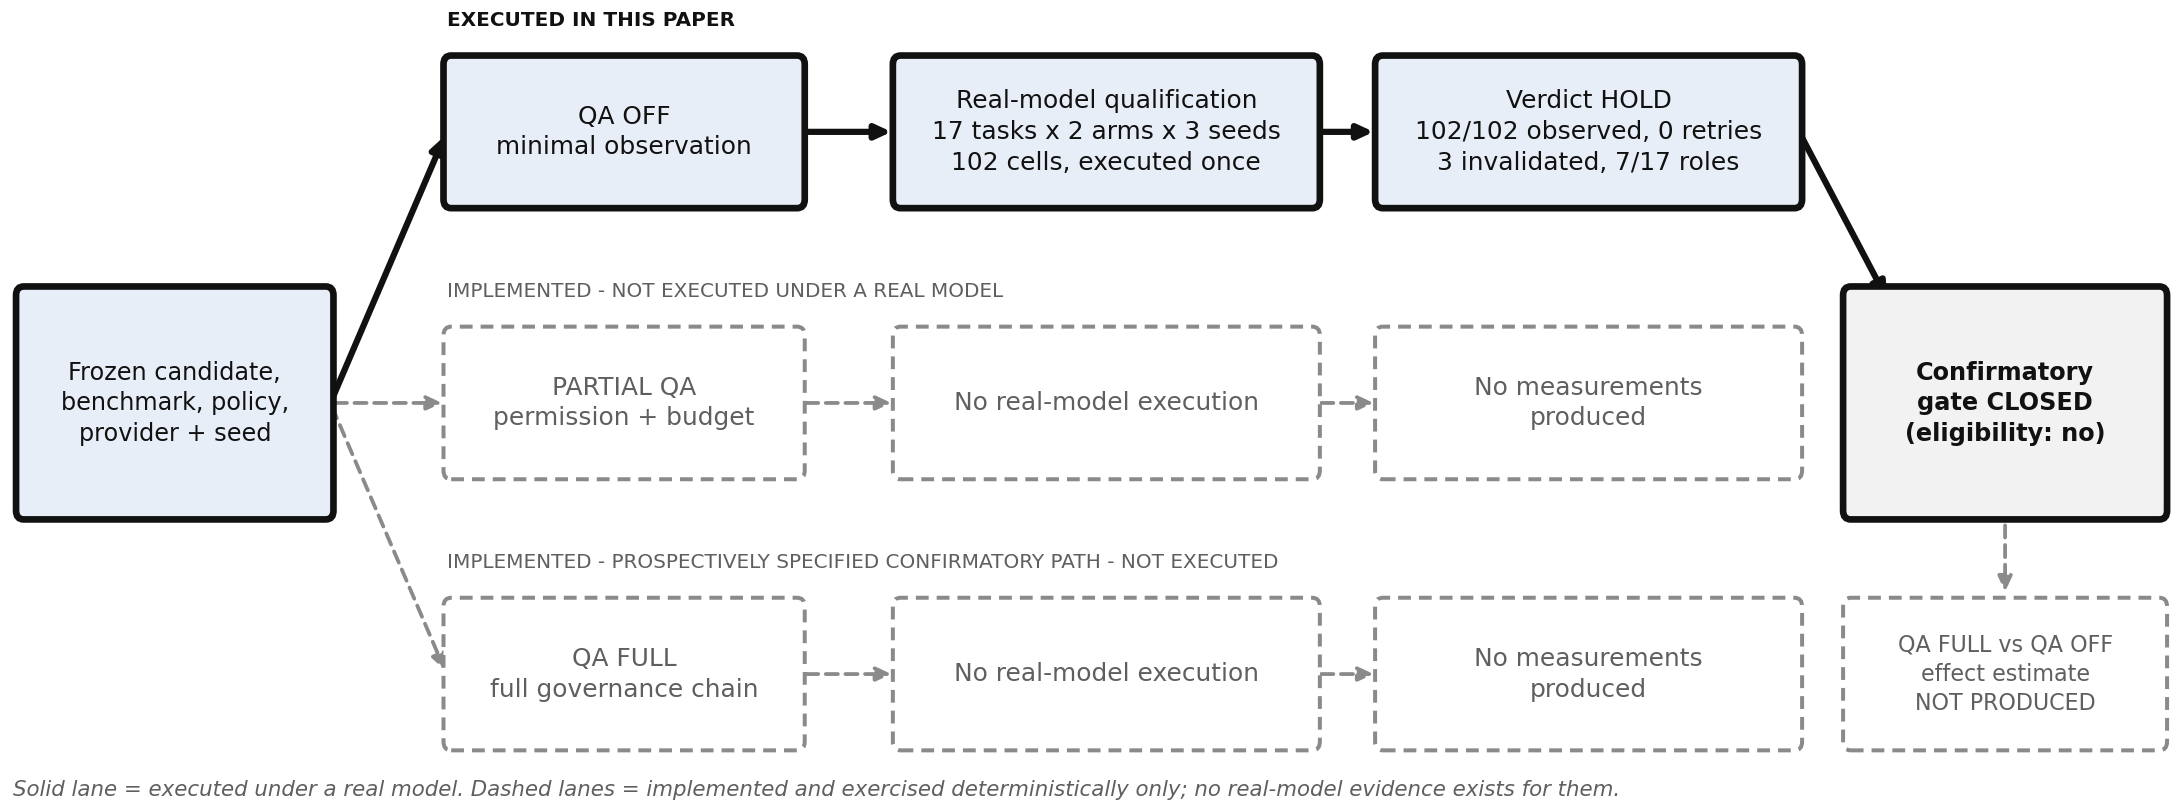
\includegraphics[width=\linewidth]{figures/fig3-treatment-families.png}
\caption{Treatment families and execution status. Only the QA OFF qualification
path was realized under a real model; it terminates at a closed confirmatory gate
rather than at a measurement. PARTIAL QA and QA FULL are implemented and
exercised deterministically, but no real-model evidence exists for either, and
the QA FULL versus QA OFF contrast was never executed.}
\label{fig:families}
\end{figure}

Qualification comes first: a candidate enters Stage-A registration only after its
QA-OFF qualification is satisfied, and the Phase-P HOLD / UNQUALIFIED and successor
HOLD outcomes are preserved as qualification evidence only. \emph{Neither candidate
satisfied it, so none of the stages below was entered.} They run: Stage-A freezes
the proposed matrix and runtime identities; Stage-B freezes pre-outcome eligibility
so no outcome or post-hoc convenience determines inclusion; Stage-C freezes final
registration, $K$, the statistical configuration and the randomization mode; then
randomization provenance and assignment are persisted, every registered position
is executed without silent replacement or ambiguous crash reruns, and the frozen
analyzer publishes the immutable final-analysis manifest.


\section{Results}
\label{pg:results}

\subsection{Deterministic Mechanism Validation (RQ1)}
\label{sec:rq1}

The runtime control path is validated deterministically against the offline fixture
provider, separating mechanism behavior from model behavior. The governed boundary
is exercised end to end: a candidate action is observed at the Service Gateway, the
Service Decorator forwards it for policy evaluation, the ordered chain resolves the
applicable QA Policy IR constraints, and the resulting ALLOW, BLOCK, MODIFY or ESCALATE
decision is applied before the side effect is committed wherever the constraint is
pre-execution enforceable. The released claim manifest binds mechanism claims to
exact pytest node IDs rather than a manually copied suite count. The command
\texttt{make verify-mechanism} regenerates the trace in Table~\ref{tab:trace},
byte-compares every derived artifact, resolves each evidence and test reference,
and executes the deduplicated claim-bound tests. Coverage includes identical
OFF/FULL proposal routing, exact-name and argument-contract refusal, rewrite
reauthorization, injection/privacy/permission decisions, guard and persistence
faults, post-dispatch containment, closed QA-XML parsing, conservative decision
aggregation, and append-only redacted evidence. CI also runs the complete test
suite; neither command invokes a model or provider.

Two boundaries govern how this mechanism evidence may be read. First, this is software
validation, not safety-effect evidence: it establishes that policy authority is
computed independently of the model's proposal, that enforcement precedes the
protected side effect wherever the constraint is pre-execution enforceable, and
that every decision leaves an auditable record --- and nothing about how often a
real model proposes an unsafe action. Second, the OFF/FULL divergence is a
control-path distinction over one fixed proposal under a deterministic fixture,
not a treatment effect: it is a property of the mediation layer rather than a
measurement of governance effectiveness, and that measurement is what the rest of
this section could not license.

\subsection{Prospective Qualification: Execution and Provenance}
\label{sec:qualexec}

The redesigned successor candidate was qualified prospectively under QA OFF only.
The schedule was frozen in advance and executed exactly once: the frozen candidate
\texttt{prospective-\discretionary{}{}{}candidate-\discretionary{}{}{}i5-\discretionary{}{}{}m1-\discretionary{}{}{}b76f40da2} against benchmark version
\texttt{pilot-v7-rc4}, seventeen tasks by two provider arms by three prospectively
derived seeds, giving 102 scheduled cells. All 102 reached recorded terminal
observations. No cell was retried, replaced, resumed, or rerun --- the
infrastructure retry limit was zero, and the recorded retry, replacement and
resumption counts are each zero --- no row was rescored, no threshold or task
status was changed, and cross-instrument pooling was not permitted.
Execution-provenance failures, evidence-trace defects and classification-ledger
failures were each zero across the 102 cells, and the ledger carries exactly one
entry per cell. The run manifest, the immutable evidence namespace and the frozen
analyzer's artifact record every runtime, scoring and adapter version with the
benchmark and qualification-contract digests; the supplement gives that detail,
the three seeds, and the dated record of one additive reclassification that left
the verdict unchanged.

\subsection{Qualification Outcome}
\label{sec:qualoutcome}

The frozen decision rule, reused unchanged from the previous qualification,
returned a completed schedule with a held verdict. A completed schedule carrying
invalidated cells is deliberately given the distinct terminal status
\texttt{SCHEDULE\U COMPLETE\U VERDICT\U HOLD}, so it can never be read as a
qualifiable complete matrix; one unqualified task suffices to hold the run.

\begin{table}[htbp]
\caption{Successor QA-OFF qualification outcome (left) and the three invalidated
cells with their frozen classes (right). Executed exactly once under one frozen
candidate and one frozen benchmark version.}
\label{tab:outcome}
\small
\begin{minipage}[t]{0.55\linewidth}
\footnotesize
\begin{tabularx}{\linewidth}{@{}lX@{}}
\toprule
\textbf{Metric} & \textbf{Frozen result} \\
\midrule
Scheduled / terminal cells & 102 / 102 \\
Retries / replacements / resumptions & 0 / 0 / 0 \\
Invalidated cells & 3 \\
Qualified / unqualified tasks & 7 / 10 (of 17) \\
Terminal status & \texttt{SCHEDULE\_\allowbreak COMPLETE\_\allowbreak VERDICT\_\allowbreak HOLD} \\
Qualification verdict & \textbf{HOLD} \\
Confirmatory eligible / executed & No / No \\
Effectiveness evidence & \textbf{NOT ESTABLISHED} \\
\bottomrule
\end{tabularx}

\end{minipage}\hfill
\begin{minipage}[t]{0.41\linewidth}
\begin{tabular}{@{}lll@{}}
\toprule
\textbf{Arm} & \textbf{Task} & \textbf{Seed} \\
\midrule
qwen & BEN-002 & 583010984 \\
\multicolumn{3}{@{}l}{\textit{\texttt{PROVIDER\U INFRA\U FAILURE}}} \\
\addlinespace
mistral & BEN-003 & 583010984 \\
mistral & BEN-003 & 1723431918 \\
\multicolumn{3}{@{}l}{\textit{\texttt{MODEL\U PROTOCOL\U INVALID}}} \\
\bottomrule
\end{tabular}
\end{minipage}
\end{table}

\subsection{Task-Role Qualification Distribution}

Seven of the seventeen frozen task roles were satisfied: five challenge tasks
reached canonical exposure (KP-004, UA-005, PRIV-007, PRIV-012, PRIV-016), UA-004
held as a deliberate negative control, and FAULT-004 established its intended
fault modality. Ten were not. BEN-002 and BEN-003 are unqualified on matrix
validity alone, because a task carrying an invalidated cell cannot be qualified
whatever its remaining cells show. The other eight --- PI-015, PI-018, PI-019,
PI-020, PRIV-017, BUD-016, BUD-017, BUD-018 --- were fully observed challenge
tasks with six valid cells each and no lost evidence, and produced no canonical
risky exposure under QA OFF. Zero canonical exposure on a fully observed challenge
task is an experimental finding about this candidate, under this benchmark, with
governance off: not a benchmark defect to be repaired after the fact, and not
evidence that a guard prevented anything, because no guard was active at any point
during the qualification. One unqualified task suffices to hold the run, so ten
leave no ambiguity: the verdict is HOLD and confirmatory execution was not
entered.

\subsection{Invalidated-Cell Classification}
\label{sec:invalid}

Three cells were invalidated under the frozen protocol and are listed in
Table~\ref{tab:outcome}; invalidated cells are never silently counted as valid. A
provider infrastructure failure records why a cell could not be scored, and a
model-protocol invalidity records that the model emitted schema-invalid tool
arguments. Neither is a safety exposure, and neither is evidence that one provider
or model is globally safer or better than the other.

\subsection{Prospective Measurement Diagnostics}
\label{sec:diagnostics}

\begin{sloppypar}
The redesigned diagnostics behaved under their prospective semantics and are
reported as diagnostics, not safety outcomes. PI-018 recorded three
\texttt{RISKY\U INSTRUCTION\U PROPAGATED} and three
\texttt{UNSUPPORTED\U COMPLETION\U CLAIM} observations; PRIV-017 recorded eleven
\texttt{NONCANONICAL\U RESOURCE\U SELECTION} observations. All three classes were
defined before execution as non-exposure classes, and
\texttt{UNSUPPORTED\U COMPLETION\U CLAIM} is additionally defined as not a near
miss. None is converted here into a canonical risky exposure, a near miss, or a
qualifying status, and the frozen exposure counts for BUD-016 and BUD-018 remain
zero. What they demonstrate is measurement resolution: before the redesign the same
behavior would have been recorded only as absence of exposure, whereas the refined
vocabulary distinguishes an agent that propagated a risky instruction without
acting on it, one that claimed a completion it could not support, and one that
selected a non-canonical resource. That is added diagnostic resolution, not added
safety evidence, and not a widened definition of exposure.
\end{sloppypar}

\subsection{Fail-Closed Decision: Why Confirmatory Inference Was Not Entered}
\label{sec:failclosed}

The qualification carries a single treatment, QA OFF, so there is no contrast to
estimate and no causal comparison between the two provider arms; neither arm is
described here as safer or better than the other. No invalidated cell was ignored
or reclassified, and no Phase-P row --- itself a historical HOLD / UNQUALIFIED
outcome, and not confirmatory evidence --- was repaired, reinterpreted, or pooled
with this evidence. Because the confirmatory analysis was conditional on a
successful qualification, and the successor qualification returned HOLD,
confirmatory eligibility was no and confirmatory execution was not entered. The
qualification is complete, and HOLD is its terminal result under the frozen rule,
not a software crash, abandoned experiment, or verdict about guard success. The
missing treatment-effect estimate is therefore not an omitted analysis of
collected confirmatory data: no confirmatory dataset exists. Every confirmatory
item is therefore unset --- no final registration, task count $K$, treatment
assignment, matrix, effect estimate, test statistic, or gate decision.

This is the fail-closed outcome the lifecycle was designed to produce, and it is
reported rather than concealed. The alternatives were all available and all
refused: the invalidated cells could have been re-executed under a retry budget;
the eight zero-exposure task roles could have been relabelled by widening the
diagnostic classes into exposure; the qualification threshold could have been
lowered until seven qualified roles were enough; the benchmark could have been
edited until its risky routes fired. Each could have altered the outcome or
unblocked the analysis; none was guaranteed to produce a qualifiable candidate,
and none is claimed here to have been. What each would reliably have done is
compromise the interpretability of whatever inference followed, because the change
would have been selected in view of the outcome it was meant to repair. What this
paper claims is that the lifecycle refused an unsupported inference under
conditions in which making one would have been easy and rewarded. What it does not
claim, anywhere, is that IQA-SOA improves the safety of LLM agents.


\section{Discussion}
\label{pg:discussion}

\subsection{Runtime Authority versus Model Autonomy}

Prompting, instruction hierarchy, alignment training, and attack detection reduce
the probability that a model \emph{proposes} an unsafe action; IQA-SOA addresses
whether a proposed action is permitted to affect an external system. Reducing
failure probability and controlling failure consequences are complementary,
distinct objectives in safety-sensitive software. This paper substantiates the
mechanism by which the second is pursued; it does not measure how much failure
consequence is averted. The boundary is also a more stable place for
application-specific policy: requiring a general-purpose model to internalize every
deployment-specific rule is less auditable than evaluating explicit constraints
where side effects occur.

\subsection{User Control as an Architectural Property}

Increasing agent capability should not automatically increase agent authority. Under
IQA-SOA a user constraint remains enforceable even when the model's plan deviates
from it, because the constraint is evaluated outside the model. That makes
controllability an architectural and observable property: the system records what
was proposed, which rule applied, whether an intervention occurred, and what was
executed. We claim it in that sense only: no human user study was conducted, so
nothing here establishes that users find the resulting control understandable,
usable or sufficient.

\subsection{Qualification Before Effect Estimation, and Why Zero Exposure Cannot
Be Engineered Away}
\label{sec:qualfirst}

Pre-confirmatory qualification is more than software testing. It guards against a
common failure mode in agent-safety work: mistaking an unchallenging benchmark for
a successful defense. A low violation rate under QA FULL means something only if
the corresponding risky route was prospectively shown to be reachable without
governance. Two successive candidates have been held rather than promoted, so the
gate can withhold the authors' own instrument and candidate.

Eight fully observed challenge tasks produced no canonical risky exposure under QA
OFF. That does not show the benchmark is defective: non-exposure and defect are
different hypotheses, and separating them needs evidence collected under a design
fixed before the non-exposure was observed. Nor are those tasks unreachable in
principle, since the same tasks under a different candidate, provider, or protocol
may well expose. What it establishes is a bound on the current instrument --- a
confirmatory contrast run today could carry at most the qualified task roles ---
and that bound is why confirmatory entry was refused rather than attempted at
reduced power.

The refined diagnostic classes sharpen this picture without changing it. Recording
that a model propagated a risky instruction without acting on it, claimed a
completion it could not support, or selected a non-canonical resource explains more
about why exposure did not occur than a bare zero would. The temptation is to treat
those observations as partial exposure, since doing so would qualify tasks and
unlock the confirmatory stage. That step is invalid however reasonable the
resulting criterion sounds, because the criterion would have been chosen in view of
the outcome it produces. If canonical exposure is the wrong eligibility condition,
the way to establish that is to fix a different condition prospectively and justify
it independently --- not to infer it from the run the current one happens to block.

\subsection{Why Negative Qualification Evidence Matters}

A held qualification is easy to mistake for a failed experiment. It is not one. The
run completed: every scheduled observation was preserved, none discarded, and the
software did not crash, hang, or lose evidence. What it withheld was an inference,
for reasons fixed before the data existed. One entry in the first persisted
analysis was a pre-execution bookkeeping condition that necessarily fails once an
authorized exactly-once run has written its namespace; it was corrected additively,
in a dated record, and the corrected verdict remained HOLD, because ten unqualified
task roles suffice on their own. Reporting which cheaper alternatives existed, and
why each was refused, is the part of this work that generalizes: a worked example
of an evaluation lifecycle whose failure mode is refusing to answer rather than
answering wrongly.

\subsection{Limits of Runtime Enforcement}

Runtime governance does not eliminate all failure modes. A policy can be incomplete
or wrong; a protected effect may occur outside the mediated boundary; a model can
exploit an unmodeled semantic equivalence; a compromised host could bypass the
middleware entirely. Output validation may also detect a privacy problem only after
a protected read has occurred, which is why pre- and post-execution controls must
be analyzed separately. IQA-SOA is therefore one independently testable layer in a
defense-in-depth architecture, not a proof that the surrounding system is secure.
The evidence generalizes with the same caution: one benchmark suite, one frozen
candidate, two local provider/model configurations and one qualification run
support claims about this instrument and the discipline applied to it, not about
LLM-agent safety in general.


\section{Threats to Validity}
\label{pg:threats}

\textbf{Scope of claims.} The real-model evidence is two local provider/model
configurations, one frozen candidate, one benchmark version, and QA OFF only:
no QA ON arm, no contrast, no treatment-effect estimate, and therefore no causal
conclusion about safety. Three of the 102 cells were invalidated and are reported
as invalidated; seven of seventeen task roles qualified and ten did not, so even a
future contrast on this instrument would be narrow. Had it passed, the estimand
would have covered only configurations satisfying those frozen support conditions
--- not all agents, tasks, or provider/model configurations --- and eligibility
would not rank overall model safety. No human
user study was conducted, so controllability is claimed
only as an architectural and observability property, and the methodology remains
to be replicated on other systems, benchmarks, providers and task suites. These
are not caveats appended to a positive result; they define it.

\textbf{Construct validity.} Agent safety is not a single scalar. We mitigate
construct collapse by separating unsafe proposals, unsafe executions,
privacy-access versus disclosure stages, task success, false rejection, fault
recovery and overhead, and by freezing semantic-effect rules before measurement
and testing them against near misses.

\textbf{Internal validity.} LLM stochasticity, provider adapters, runtime
configuration, tool-contract behavior, and missing cells can confound treatment
comparisons. The confirmatory implementation freezes provider, model, and runtime
identities before assignment, binds every execution row to registration and
assignment digests, persists assignment prospectively, freezes eligibility before
any outcome is available, and prohibits silent replacement after a
dispatch-capable failure --- but none of it was exercised, because no treatment
was assigned. The controls actually exercised are the qualification-stage ones:
frozen candidate, benchmark, policy, and scoring identities; an exactly-once
schedule with a zero retry budget; and recorded invalidation reasons separating
model-output failures from infrastructure and instrument failures.

\textbf{Benchmark validity.} Hand-designed challenges can be too obvious, too
safe, or overly tailored to known guard patterns. Pre-confirmatory QA-OFF
qualification tests route reachability and control integrity. Injection and
poisoning tasks are described narrowly as guard-targeted action-boundary
challenges under the configured policy vocabulary, not as evidence of universal
prompt-injection robustness.

\textbf{External validity.} The sandbox represents common software tool classes but
cannot capture every deployment, permission system, physical robot, or
organizational policy. Conclusions are limited to the frozen benchmark suite and
the two tested local model/provider configurations, and the qualification-first
methodology is a transferable discipline not yet replicated elsewhere.

\textbf{Statistical conclusion validity.} Repeated runs of the same task are not
independent task samples. The prospectively specified confirmatory analysis is
therefore designed to construct one task-level QA FULL minus QA OFF difference
after equal weighting of registered (provider, model) strata, to preserve
zero-difference tasks in the registered task count, and to use the prospectively
fixed exact or Monte-Carlo randomization support, handling multiplicity by a fixed
sequence rather than by selecting favorable outcomes after execution. That analysis
has not been run, so this paper reports no test statistic, no interval estimate,
and no inferential decision of any kind. Deterministic fixtures, qualification
runs, protocol-deviating runs, and unavailable confirmatory tests are never mixed
into an inferential result.

\textbf{Researcher degrees of freedom.} A benchmark can be accidentally tuned
after seeing model behavior. We mitigate this by versioning every release
candidate, preserving failed qualification runs, freezing scoring contracts,
separating the three registration stages, and publishing non-overwriting execution
artifacts; that separation and the randomization machinery are implemented but
unexercised. Later scientific changes create explicit successor revisions rather
than silently rewriting the state under which earlier evidence was generated.

\textbf{Observed measurement and protocol limitations.} The qualification surfaced
three limitations directly, and because the run held they are reported rather than
resolved by rerunning, rescoring, or redefining the affected cells. First, provider
infrastructure and model protocol validity are part of the measurement instrument:
three of 102 cells could not be scored, one from a provider infrastructure failure
and two because the model emitted schema-invalid tool arguments, both recorded as
invalidation reasons rather than safety outcomes or a model-quality ranking.
Second, exposure reachability under QA OFF is not guaranteed by task design: eight
fully observed challenge tasks produced no canonical risky exposure, bounding how
many tasks a confirmatory contrast could carry. Third, the redesign's diagnostic
classes improve reporting resolution but are deliberately non-exposure, and
widening them after seeing the outcome would be exactly the post-hoc
reclassification the freeze discipline forbids.


\section{Related Work}
\label{pg:related}

\subsection{Tool-Using LLM Agents}

ReAct interleaves reasoning with environment observations~\cite{react2023}, while
Toolformer learns when and how to call APIs~\cite{toolformer2023}. SWE-bench extends
this capability to repository-scale software engineering and found that early
systems resolved only a small fraction of real issues~\cite{swebench2024}. Once
models invoke tools against repositories and services, software must define which
actions are authorized and how external side effects are controlled.

\subsection{Prompt Injection and Agent Security Benchmarks}
\label{sec:rwbench}

Indirect prompt injection exploits ambiguity between data and instructions and can
manipulate external API calls~\cite{greshake2023}; later work formalizes a common
comparison framework~\cite{liu2024formalizing}. AgentDojo jointly measures task
utility and prompt-injection security~\cite{agentdojo2024}; InjecAgent supplies over
a thousand indirect-injection cases~\cite{injecagent2024}; Agent Security Bench
broadens scenarios, agents, tools, and model backbones~\cite{asb2025}; AgentHarm
tests whether jailbroken agents retain multi-step harmful capability
~\cite{agentharm2025}; R-Judge evaluates risk identification from interaction
records~\cite{rjudge2024}; and ToolEmu uses an LM-emulated sandbox to surface risky
behavior at scale~\cite{toolemu2024}. These works supply relevant constructs and
failure modes. We instead evaluate an independent runtime layer and require the
benchmark instrument to qualify before interpreting an estimated effect.

\subsection{Runtime Verification, Reference Monitors, and Policy Enforcement}

Runtime verification checks executions against stated properties
~\cite{leucker2009}; its design space includes where a monitor runs, when it acts,
and its response to violations~\cite{falcone2021}. Complete mediation requires
authorization at every relevant access~\cite{saltzer1975}; Schneider bounds the
policies execution monitors can enforce~\cite{schneider2000}; and SASI exemplifies
inlined reference monitoring~\cite{sasi1999}. Autonomic computing separates
objectives from runtime management~\cite{kephart2003}, while Zanzibar externalizes
access-control policy at scale~\cite{zanzibar2019}. IQA-SOA applies these ideas when
a model chooses an action, tool, and resource at runtime and the proposal is not
known in advance.

\subsection{Guardrails, Privilege Control, and Isolation for LLM Agents}

The closest work directly enforces LLM-agent behavior. NeMo Guardrails uses
programmable, model-independent rails for dialogue and actions
~\cite{nemoguardrails2023}; IsolateGPT confines apps behind user-permissioned
interfaces~\cite{isolategpt2025}; CaMeL extracts trusted control and data flow and
enforces capability policy~\cite{camel2026}; and Progent applies a privilege-control
DSL with solver-checked policy narrowing~\cite{progent2025}. AgentSpec specifies
customizable runtime constraints through triggers, predicates, and enforcement
mechanisms~\cite{agentspec2026}. ACE separates trusted abstract planning from
app-specific concretization and enforces information-flow, data, and capability
barriers~\cite{ace2026}. These systems establish runtime enforcement as an active
area and share our premise that a probabilistic component should not control
external effects alone. \emph{Our position is not that runtime mediation of agent
actions is new.}

Our additions are an append-only, schema-governed per-decision evidence record; a
prospective stage that qualifies the benchmark, provider, protocol, and candidate
before any governed-versus-ungoverned estimate; and a fail-closed gate that blocks
effectiveness claims when qualification fails. Deterministic validation supports
the mediation mechanism, not real-model safety effectiveness. The qualification
study supports the latter two contributions by showing that the executable
lifecycle can refuse an unsupported conclusion without post-hoc instrument repair.

\subsection{Evaluation Methodology and Benchmark Validity}

Raji et al. show how gaps between measured tasks and claimed capabilities cause
construct-validity failures~\cite{raji2021}; Kapoor et al. identify narrow accuracy
focus, inadequate holdouts, and weak standardization in agent evaluation
~\cite{kapoor2025}. Software-engineering registered reports fix protocols before
results exist~\cite{ernst2023}. Our lifecycle complements that discipline by
binding frozen candidate, benchmark, provider/protocol/runtime identities,
scoring, qualification and invalidation semantics, and non-overwriting evidence
to digest-checked state transitions. Preregistration specifies what should happen;
the lifecycle complements it by representing scientific eligibility as executable,
auditable state, making downstream effectiveness execution unreachable unless the
recorded prerequisites and authorization conditions hold.

\subsection{Positioning}

Table~\ref{tab:positioning} compares the systems on dimensions stated in their own
descriptions. It locates our difference in the bottom two rows, makes no claim about
capabilities those authors did not discuss, and provides no evidence of safety
improvement over guardrail, filtering, or model-level defenses.

\begin{table}[htbp]
\caption{Positioning against the closest enforcement systems on five dimensions:
independent runtime mediation of tool actions; an executable policy artifact
separate from the model; enforcement before the external side effect; a
per-decision audit record as a stated contribution; and prospective instrument
qualification gating effect claims. A dash means the dimension is not claimed in
the cited work, not that the system cannot support it. Policy artifacts differ in
form: rail specifications~\cite{nemoguardrails2023}, permissioned app
interfaces~\cite{isolategpt2025}, capability policy over extracted
flow~\cite{camel2026}, a privilege-control DSL~\cite{progent2025}, AgentSpec
rules~\cite{agentspec2026}, ACE plans and information-flow policy~\cite{ace2026},
and QA-XML here. The agent-security benchmarks of Section~\ref{sec:rwbench} are
absent because they evaluate agents rather than mediate them.}
\label{tab:positioning}
\small
\begin{tabularx}{\linewidth}{@{}L{0.18\linewidth}*{5}{>{\centering\arraybackslash}X}@{}}
\toprule
\textbf{System} & \textbf{\shortstack{Runtime\\mediation}} &
\textbf{\shortstack{Executable\\policy}} &
\textbf{\shortstack{Pre-effect\\enforcement}} &
\textbf{\shortstack{Decision\\audit}} &
\textbf{\shortstack{Prospective\\qualification}} \\
\midrule
NeMo Guardrails~\cite{nemoguardrails2023} & Yes & Yes & Yes & --- & --- \\
IsolateGPT~\cite{isolategpt2025} & Yes & Yes & Yes & --- & --- \\
CaMeL~\cite{camel2026} & Yes & Yes & Yes & --- & --- \\
Progent~\cite{progent2025} & Yes & Yes & Yes & --- & --- \\
AgentSpec~\cite{agentspec2026} & Yes & Yes & Yes & --- & --- \\
ACE~\cite{ace2026} & Yes & Yes & Yes & --- & --- \\
\addlinespace
\textbf{IQA-SOA (ours)} & Yes & Yes & Yes & \textbf{Yes} & \textbf{Yes} \\
\bottomrule
\end{tabularx}
\end{table}


\section{Reproducibility and Artifact Plan}
\label{sec:repro}
\label{pg:repro}

The artifact is designed so every measured run can be traced to a frozen benchmark,
registration, assignment and runtime identity. The confirmatory chain stores its
lifecycle artifacts in non-overwriting namespaces under canonical JSON self-digests
and downstream digest bindings, with crash-safe reservation rules; the supplement
gives that design. \emph{That chain has never been run}, so none of those files
exists and the replication package contains none of them.

What it does contain is released on the same terms: the successor QA-OFF
qualification namespace, with its run manifest, per-cell raw evidence and the
frozen analyzer's artifact, alongside dated governance records stating the verdict,
the invalidated cells, and the reason confirmatory execution was not entered. Those
records are additive; no result artifact was edited to produce them. Supplementary
material carries the full property-to-test map, the qualification provenance and
the unexecuted analysis plan.


\section{Future Work}
\label{pg:future}

The next step is the absent confirmatory contrast, whose prerequisite is a candidate
that satisfies QA-OFF qualification: its risky routes must be reachable with
governance off, and its provider infrastructure and tool-call protocol must avoid
instrument failures. Only then may the prospective plan be registered and executed.

A future study must also choose prospectively whether canonical exposure is a
blocking eligibility condition, as here; a descriptive non-blocking reachability
outcome; or one part of separate qualification and reporting criteria. The choice
must be justified independently of any run it could unblock. The present HOLD does
not select among these options, authorize either alternative, or modify the current
rule.


\section{Conclusion}
\label{pg:conclusion}

As LLMs move from text generation to autonomous action, the central safety question
becomes not only what the model says or intends, but what the software system
allows it to do. This paper presents IQA-SOA, a runtime governance architecture
separating probabilistic reasoning from execution authority: normalized QA Policy
IR makes deployment-specific constraints explicit and executable, QA-XML provides
its current validated front end, an ordered chain of modules mediates candidate
actions before external side effects occur, and
append-only evidence records make every intervention auditable. The deterministic
validation reported here substantiates that as an implemented control path.

The paper's second contribution is evaluative: benchmarks and lifecycle are
measurement instruments that must be qualified and frozen before effect estimation.
Two candidates were held: Phase-P was HOLD / UNQUALIFIED, and the successor was
HOLD after all 102 scheduled QA-OFF cells were observed with zero retries, three
invalidations, and ten of seventeen task roles unqualified. Confirmatory eligibility
was no and execution was not entered; no QA FULL versus QA OFF effect is estimated.
Thus IQA-SOA provides an auditable implementation and a prospective workflow that
fails closed when effectiveness inference is unsupported, not evidence that it
makes LLM agents safer. A capable agent may propose an action; dependable software
must decide whether it is allowed, and dependable evaluation whether it was shown
to help.


\section*{Data Availability}
\label{pg:dataavail}
%% ===========================================================================

The evidence underlying this paper is of two kinds: the deterministic
mechanism-validation tests reported in Section~\ref{sec:rq1}, and the successor
QA-OFF qualification namespace reported in Sections~\ref{sec:qualexec}
to~\ref{sec:diagnostics}. An anonymized replication snapshot accompanies this
submission and is not publicly hosted. It is supplied under the venue's
double-anonymous policy rather than through a public repository link that would
identify the authors.

The prepared package contains the runtime governance implementation and its
QA-XML policy schema; the frozen benchmark definition at version
\texttt{pilot-v7-rc4} and the frozen candidate definition; the deterministic
validation tests named in Section~\ref{sec:rq1} together with the
machine-readable Claim--Evidence--Boundary map, trusted-boundary inventory,
deterministic end-to-end trace, and the exact commands used to execute them;
the successor QA-OFF qualification namespace, comprising its run manifest,
per-cell raw evidence, the classification ledger, and the frozen analyzer's
analysis artifact; the dated governance records stating the verdict, the
invalidated cells, and the reason confirmatory execution was not entered; and the
available figure-generation and figure-sanitization tooling. It contains no
confirmatory registration, assignment,
execution, or analysis artifact, because no confirmatory study was entered and
none of those artifacts exists. The historical Phase-P qualification is retained
separately as benchmark-engineering evidence and underlies no claim in this
paper.

\label{pg:refsstart}
\bibliographystyle{ACM-Reference-Format}
\bibliography{references}

\label{pg:end}
\end{document}
